\begin{frame}{Gadżety}
\begin{columns}
    \begin{column}{0.4\textwidth}
    Definiujemy relację w grafie przy~pomocy:
        \begin{itemize}
            \item relacji krawędzi: \(\longleftrightarrow\)
            \item koniunkcji: \(\land\)
            \item równości wierzchołków: \(=\)
            \item kwantyfikatora: \(\exists\)
        \end{itemize}
    \end{column}
    \begin{column}{0.6\textwidth}
    \begin{figure}
        \centering
        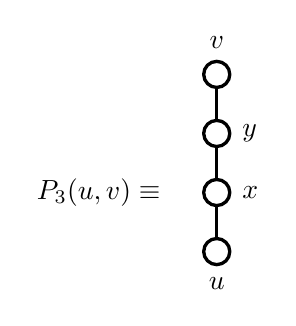
\begin{tikzpicture}[
    scale=0.5,
    line width=1.2pt
]
\onslide<2->{
    \node at (-7,-3) {\(P_3(u,v)\equiv\)};
    
    \node[circle, draw=black, fill=white, label=below:{\(u\)}]
            (p0) at (-4,-4.5) {};

    \node[circle, draw=black, fill=white, label=right:{\(x\)}]
            (p1) at (-4,-3) {};
    \node[circle, draw=black, fill=white, label=right:{\(y\)}]
            (p2) at (-4,-1.5) {};

    \node[circle, draw=black, fill=white,
    label=above:{\(v\)}]
        (p3) at (-4,0) {};
    

    \draw (p0) -- (p1);
    \draw (p1) -- (p2);
    \draw (p2) -- (p3);
}
\end{tikzpicture}
    \end{figure}
        \onslide<2->{
        \[P_3(u,v)=\exists_{x,y} \ u \leftrightarrow x \land x \leftrightarrow y \land y \leftrightarrow v\]
    }
    \vspace{-2em}
    \end{column}

\end{columns}
\end{frame}